\chapter{Workflow \textit{as is} na notação BPMN}\label{cap:workflow-bpmn}

Este capítulo documenta o processo de negócio vigente na operação de coleta e entrega analisada, na situação em que se encontra antes da adoção do S.R.I. A descrição é apresentada na notação BPMN e serve de referência para a identificação das atividades manuais que o sistema se propõe a substituir \cite{omg2011bpmn}.

A representação do processo atual, denominada \textit{as is}, tem por finalidade explicitar não apenas a sequência das atividades, mas também a responsabilidade de cada participante e os pontos de troca de informação entre eles. Essa explicitação é o que permite reconhecer, de forma objetiva, quais etapas agregam valor à operação e quais decorrem de limitações das ferramentas empregadas \cite{omg2011bpmn}.

\section{Descrição do processo atual}

O processo atual está organizado em duas raias, que identificam os dois participantes envolvidos na operação: o Atendente, responsável pelo registro do pedido de coleta e pela organização das informações, e o Motorista, responsável pela execução do deslocamento e pela efetivação da coleta e da entrega. O diagrama correspondente é apresentado na Figura \ref{fig:workflow-as-is}.

O processo inicia-se na raia do Atendente, com a atividade \textit{Receber Pedido de Coleta}, na qual são obtidas do solicitante as informações necessárias ao atendimento. Em seguida, o Atendente executa a atividade \textit{Marcar no Quadro}, registrando manualmente, em um quadro de anotações, os dados recebidos. Esse registro constitui, na prática, a única forma de armazenamento das informações da operação.

Concluído o registro, tem início, já na raia do Motorista, a atividade \textit{Coletar Informações do Quadro}, na qual o Motorista precisa recuperar, a partir das anotações, os endereços e as demais informações referentes às coletas que lhe foram atribuídas. Como as anotações são feitas em um quadro físico, sem estrutura de dados que associe cada pedido ao seu solicitante, essa recuperação exige a leitura e a interpretação do conjunto de registros, o que introduz dependência da presença física do Motorista junto ao quadro e abre espaço para erros de transcrição e de identificação.

A etapa seguinte é a atividade \textit{Preparar Rota}. Nela, o Motorista define manualmente a ordem em que as coletas serão realizadas e elabora o trajeto correspondente, sem apoio de qualquer ferramenta de otimização. A decisão baseia-se na experiência prévia do profissional e no conhecimento que ele possui da região, o que faz com que a qualidade do trajeto varie entre motoristas e dependa da memorização de percursos anteriores.

Definida a sequência, o Motorista executa a atividade \textit{Realizar Coleta}, deslocando-se até cada ponto anotado e efetuando a coleta dos itens. Cada deslocamento entre pontos é planejado de forma isolada, uma vez que o quadro não oferece qualquer recurso de ordenação ou de visualização geográfica das paradas. Encerradas as coletas, executa-se a atividade \textit{Entregar na Agência}, que fecha o processo com o retorno do material ao ponto de origem.

\begin{figure}[p]
    \centering
    \caption{Workflow \textit{as is} do processo de coleta e entrega}
    \label{fig:workflow-as-is}
    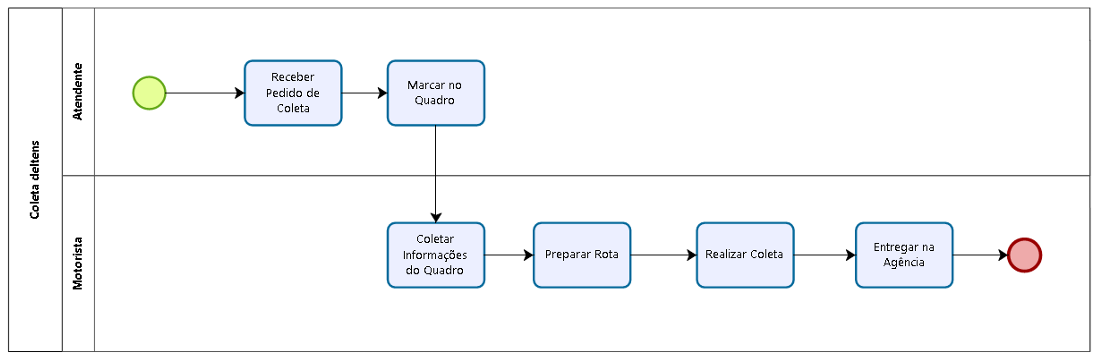
\includegraphics[angle=90,width=21cm]{imagens/workflow-as-is.png}
    \vspace{2pt}
    \footnotesize Fonte: o próprio autor (2026)
\end{figure}

\section{Ineficiências identificadas}

A análise do processo descrito permite identificar quatro ineficiências estruturais que o S.R.I. se propõe a resolver.

A primeira é a ausência de armazenamento estruturado das informações. O quadro de anotações não constitui um repositório consultável: os dados não são indexados por solicitante, não preservam histórico e não permitem busca por endereço ou por data. Essa característica obriga o registro manual repetido dos mesmos dados a cada novo pedido e impossibilita o reaproveitamento das informações em operações futuras.

A segunda é a dependência do quadro físico como intermediário. A atividade de coletar informações do quadro só pode ser executada com o Motorista presente junto às anotações, o que cria um acoplamento entre a etapa de registro e a etapa de execução que não tem correspondência com as necessidades da operação. Esse acoplamento também é a origem de erros de transcrição, uma vez que a transferência das informações ocorre por leitura humana.

A terceira é a elaboração manual da rota. Como não há ordenação automatizada das paradas, a sequência definida pelo Motorista tende a priorizar a ordem em que as coletas foram registradas ou a familiaridade com determinada região, e não a minimização da distância total percorrida. O resultado é a ocorrência de deslocamentos redundantes e de cruzamentos desnecessários de trajeto, com efeito direto sobre o consumo de combustível e sobre o tempo de operação.

A quarta é a inexistência de reutilização de trajetos. Mesmo quando a operação diária repete a mesma sequência de pontos, o processo não prevê qualquer mecanismo de armazenamento da rota definida, de modo que a atividade de preparar a rota é integralmente refeita em cada jornada. Essa repetição consome tempo de trabalho que poderia ser dedicado ao deslocamento e à entrega, além de impedir que o conhecimento acumulado pelo profissional seja preservado.

\section{Relação com a solução proposta}

Cada uma das ineficiências identificadas corresponde a um requisito do S.R.I. A ausência de armazenamento estruturado é endereçada pelo módulo de gerenciamento de locais, que substitui o quadro por registros persistidos no banco de dados local do aplicativo, indexados por identificador e pesquisáveis por nome \cite{sriEspecUC2026}. A dependência do quadro físico é eliminada pela portabilidade do dispositivo móvel, que disponibiliza as informações do local em qualquer ponto de operação, com a localização do ponto representada sobre o mapa.

A elaboração manual da rota é substituída pela funcionalidade de geração de rotas, que ordena as paradas a partir das coordenadas dos locais cadastrados e calcula o trajeto sobre a malha viária. A inexistência de reutilização de trajetos é resolvida pelo módulo de rotas salvas, que preserva o trajeto calculado e permite reexecutá-lo em outra data. Desse modo, o desenho do sistema mantém correspondência direta com o processo documentado, o que reforça a rastreabilidade entre a análise do negócio e os requisitos de software \cite{sriEspecComp2025}.
